\documentclass[11pt]{article}
\usepackage{amsmath,amsfonts,latexsym,graphicx}
\usepackage{fullpage}
\usepackage{url,hyperref}
\usepackage{subfig}
\usepackage{tikz}
\usetikzlibrary{arrows,decorations.pathmorphing,backgrounds,fit,shapes.geometric}
\usepgflibrary{shapes.geometric}
%\usepackage{ijcai09}

\pagestyle{empty}

\setlength{\oddsidemargin}{0in}
\setlength{\topmargin}{0in}
\setlength{\textwidth}{6.5in}
\setlength{\textheight}{8.5in}

\newtheorem{fact}{Fact}[section]
\newtheorem{lemma}{Lemma}[section]
\newtheorem{theorem}[lemma]{Theorem}
\newtheorem{assumption}[lemma]{Assumption}
\newtheorem{definition}[lemma]{Definition}
\newtheorem{corollary}[lemma]{Corollary}
\newtheorem{prop}[lemma]{Proposition}
\newtheorem{claim}[lemma]{Claim}
\newtheorem{remark}[lemma]{Remark}
\newtheorem{prob}{Problem}
\newtheorem{conjecture}{Conjecture}


\newenvironment{proof}{\vspace{-0.15in}\noindent{\bf Proof:}}%
        {\hspace*{\fill}$\Box$\par}
\newenvironment{proofsketch}{\noindent{\bf Proof Sketch.}}%
        {\hspace*{\fill}$\Box$\par\vspace{4mm}}
\newenvironment{proofof}[1]{\smallskip\noindent{\bf Proof of #1.}}%
        {\hspace*{\fill}$\Box$\par}

\newcommand{\etal}{{\em et al.}\ }
\newcommand{\assign}{\leftarrow}
\newcommand{\eps}{\epsilon}

%\newtheorem{lemma}{Lemma}
%\newtheorem{theorem}[lemma]{Theorem}
\begin{document}

\title{Information Set Generation in Kriegspiel}
\author{Abhishek Gupta\qquad Mark Richards\qquad Osman Sarood\\University of Illinois at Urbana-Champaign\\CS598LVK:
Parallel Combinatorial Search} \maketitle

\begin{abstract}
Information Set Generation is the identification of the set of paths in an imperfect information game tree that are
consistent with a player's observations.  The ability to reason about the possible state of the world is crucial to the
performance of game playing agents.  In this work, we discuss the problem of information set generation in the context
of kriegspiel (partially observable chess).  We implement the algorithm on top of a general purpose combinatorial search
engine and discuss its performance under different load balancing strategies and with different grainsize parameters.
We discuss some variations in the search strategy and their effect on performance.  \end{abstract}

\section{Introduction}
In imperfect information games, players do not have access to full knowledge of the world. Examples of imperfect
information include hidden cards in Poker~\cite{billings02challenge} or Bridge~\cite{ginsberg96partition}, hidden tiles
in Scrabble~\cite{richards07opponent}, or hidden pieces in Stratego or Kriegspiel (partially observable
chess)~\cite{li94chess}. The game tree nodes that are indistinguishable to a player because they differ only in the
information that is hidden to the player by rule are called that player's {\em information set.}  The ability to
estimate the value of the possible states and to reason about the probability distribution over those states is crucial
to playing imperfect information games well. 

The term {\em belief state} is sometimes used interchangeably with information set to refer to a probability
distribution over possible worlds.  The latter term comes from the game theory community and is preferred here.  A node
in a game tree denotes not only the current state of the game, but also uniquely defines a path from the initial state
or root node.  Thus, a game tree node implicitly encodes not only the current state of the game, but also all the
history of all decisions made by all players up to that point in the game.  Knowing one's information set means knowing
all possible game histories.

For many games, solving the information set generation problem is trivial.  For example, in a poker game, it is easy to
see that the unseen cards held by a player's opponents may be any permutation of the cards not seen by that player
(i.e., hole cards and any revealed community cards).  After the betting rounds, it would not be reasonable to assume
that each of these permutations of unseen cards is equally probable, as betting decisions made by the players up to that
point would be affected by the quality of those players' cards.  But the set of {\em possible} hands for all of the
opponents is easy to conceive and enumerate.

In the game of kriegspiel, information set generation is non-trivial.  The player knows the opponent's position with
certainty when the game begins, but after the initial move there may be varying levels of uncertainty about the location
of the opponent's pieces.  Unlike poker, it is not possible to simply permute all of the opponent's possible pieces over
all of the squares not occupied by the player's own pieces.  A configuration of pieces for the opponent is only valid.
Information set generation is not the same problem as solving a game tree, although it is arguably a necessary
subroutine for quality game play in imperfect information games. The standard game tree problem is to find an
equilibrium (i.e., minimax) strategy for the game. This can be done using alpha-beta pruning for perfect information
games or linear programming for imperfect information games. Information set generation, by contrast, is the problem of
finding sequences of moves in the game tree that are consistent with a player's observations.

\section{Background}
In this section, we describe the game of kriegspiel, and the particular variation of it that we have implemented.

Kriegspiel was invented in the 1800s.  Historically, the game has required three parties: two competing players and one
referee.  Each player sits with a chessboard that is partitioned off so as not be seen by the others.  One player
controls the white pieces; the other controls the black pieces.  The referee keeps track of both sets of pieces.  Each
player has a full set of chess pieces.  He may position the opponent's pieces however he wishes on his own board (if at
all).  The players alternate moves as in a regular chess game, but instead of announcing their moves out loud, they
write the source and destination square of their desired play son a piece of paper and pass them to the referee, so that
the move is not heard by the other player. The referee, who knows the location of all pieces, checks the legality of the
move.  If the move is legal, the referee makes the move on his own board and announces that a legal move has been made
and that it is the other player's turn to move.  If the move is illegal because it is blocked by an opponent's piece or
would place or leave the active player in check, the referee announces, "No."  There is no penalty for attempting an
illegal move.  The player continues to attempt moves until one finally succeeds.  If a player has no legal moves
(because of stalemate or checkmate), the referee announces the game's result.  With the advent of computers, it is
convenient to play the game over a network, with a computer acting as the referee.

The referee makes other announcements besides declaring move illegal, and there are several variations of the game that
differ only in the nature of these announcements.  All declarations by the referee are heard by both players.  Thus, for
example, a player will hear and know if her opponent has attempted an illegal move, and will thus know that her
opponent's pieces are configured in such a way as to allow at least one attemptable move that blocked or would leave him
in check.  

The referee announces when a player is in check.  (And again, this announcement is heard by both players.)  There is
some variation in what additional information is supplied in this case.  In one popular variant, the referee declares
that the player is in check "by rank," "by file," "by diagonal," or "by knight."  In the case of a diagonal attack, the
referee may announce whether the checking piece is along the long or short diagonal (from the king's perspective).  It
is possible to be in check by two pieces at the same time, in which case the direction of both attacks would be
declared.  In our implementation, for simplicity, the referee declares only that the player is in check, without
specifying the nature of the attack.

In the case of the capture, the referee announces the location of the piece that was captured, so that both players can
remove the piece from the board.  In some variations, the referee also announces whether the captured piece was a pawn
or non-pawn.  In our implementation, information about the captured piece is not explicitly provided to the player who
makes the capture.

Because there is no penalty for making illegal moves, it is often to a player's advantage to attempt to make moves which
are likely to be illegal, as hearing such declarations from the referee can provide important information to a player
about the location of the opponent's pieces.  In particular, since a diagonal move by a pawn is legal only the case
where such a move would capture an opponent's piece, it could potentially be profitable to attempt all or many pawn
captures on every turn.  In order to speed the game up, popular variants of the game require the referee to make some
kind of declaration at the beginning of a player's turn with respect to the pawn captures that are available.  This may
be as simple as declaring "Try" to indicate that at least one pawn capture is possible.  In our implementation, the
referee declares all possible pawn captures.

In the case of a pawn promotion, the player making the pawn advancement would secretly notify the referee as to which
piece (queen, rook, bishop, or knight) he would like.  To reduce the number of bits needed to specify a move, our
implementation assumes and allows only promotion to queen. 

In general, any move that is legal in a regular chess match may be at least attempted by a player in kriegspiel.  And
any kriegspiel move that is ultimately allowed by the referee would also be a legal move in chess.    

We assume that a player may not attempt the same illegal move more than once per turn.  This means that if a player
hears multiple declarations from the referee that the opponent has attempted an illegal move, the player may assume that
the opponent has at least that many possibilities available to him.

\subsubsection{Special Moves}
Our implementation supports the capability for pawns to move two spaces on their first turn.  However, we did not
implement support for castling or {\em en passant} pawn capture. 

\subsection{Example}
The concept of information sets is perhaps best explained through an example.  Figure~\ref{listing} shows a full listing of an
actual kriegspiel game from ~\cite{li94chess}.  We have adapted the notation used by Wolfe for Berkeley Kriegspiel.  The
moves are numbered in pairs: a move by white on one line followed by black's move on the next line.  The actual move is
shown first followed by a list of referee announcements.  Captures announcements are prefixed with an X and give the
location of the captured piece.  Similarly, pawn tries announcements are prefixed with T.  Attempted moves that were
ultimately declared illegal are shown in a list following the ':'.  For example at move 9, (Figure~\ref{fig:9W}--\ref{fig:9B}), black
attempts to block a potential threat along the diagonal by moving a pawn to f6, then attempts to escape or capture a
threat at f7.  When both of these attempts fail, black can infer that his king is being threatened by a protected bishop or
queen at f7.  The attempt to move to e7 is black's way of finding out whether the threatening piece is a queen or
bishop.  When this move fails, black knows it is white's queen and ultimately retreats to d8.  Note that the failed
moves by white on turns 3 and 4 are a result of being blocked by the pawn at e2.

\begin{figure}
\begin{verbatim}
1. d4 {(:)}
   a5 {(:)}
2. Bg5 {(:)}
   b6 {(:)}
3. Nc3 {(:Bd8)}
   c5 {(:)}
4. d5 {(:Bd8;Tc5)}
   Na6 {(:)}
5. d6 {(:)}
   f6 {(:Td6)}
6. e4 {(:)}
   fxg5 {(Xg5:Td6;Tg5)}
7. Bc4 {(:)}
   exd6 {(Xd6:Td6)}
8. Qd5 {(:)}
   Qc7 {(:)}
9. Qf7+ {(:)} 
   d8 {:g6,f7,e7}
10. Qxf8++ {(1-0:)}
\end{verbatim}
\caption{Listing of a kriegspiel game resulting in checkmate by white after 10 moves.}
\label{listing}
\end{figure}


Note that the listing in Figure~\ref{listing} corresponds to the referee's view of the game and would be useful for
post-game analysis or commentary.  During the game, players would not have access to the full information.  The
transcript from white's perspective is shown in Figure~\ref{filteredlisting}.  Note that black's actual moves have been
replaced with ``??'' and lists of black's illegal moves have been replaced with the {\em number} of illegal attempted
moves.  For example, on move 9, black attempted three illegal moves.
\begin{figure}
\begin{verbatim}
1. d4 {(:)}
   ?? {(:0)}
2. Bg5 {(:)}
   ?? {(:0)}
3. Nc3 {(:Bd8)}
   ??  {(:0)}
4. d5 {(:Bd8;Tc5)}
   ??  {(:0)}
5. d6 {(:)}
   ?? {(:0,Td6)}
6. e4 {(:)}
   fxg5 {(Xg5:Td6;Tg5)}
7. Bc4 {(:)}
   ?? {(Xd6:Td6)}
8. Qd5 {(:)}
   ?? {(:0)}
9. Qf7+ {(:)} 
   ?? {:0}
10. Qxf8++ {(1-0:)}
\end{verbatim}
\caption{Listing of a kriegspiel game resulting in checkmate by white after 10 moves.}
\label{filteredlisting}
\end{figure}

   
 

\section{Related Work}
In this work, we have argued for an information set generation approach to kriegspiel, but other authors have approached
the problem differently.  Parker \etal, consider the problem of sampling from belief states in a variety of large
game trees, including kriegspiel~\cite{parker05game}.  They show that some performance gains can be achieved by only
approximate sampling from the belief state.  Instead of generating the full information set, or even sampling from it,
they sample from possible positions for the current state (i.e., sampling from the belief state) by matching only the
most recent observations.  This motivation for this approach seems to be that it would not be feasible to sample from
the full information set, because of the computational expense involved.  And indeed, our experiments bear this out-- it
can indeed be expensive to produce the full information set.  For the experiments shown in Table XX, generating the full
information set took over 25 minutes on a single processor.  However, by utilizing the Charm++ search engine on a
parallel machine (1024 processors), we were able to generate the full set in just 2.9 seconds.  (Note that this set had
more than 4 million members.)  Our results suggest that the problem is highly scalable and our approach might therefore
be preferred.

Li gives an overview of kriegspiel and discusses strategy from the perspective of human players~\cite{li94chess}.  He
walks through the analysis of several actual games between two human players and discusses the inferences that each
player can and should make at each position.  As in chess, human players are able to reason about the game at an
abstract level; they tend to focus on a small number of critical possibilities and to emphasize the most important
pieces and squares in each position.  Computer agents, lacking such sophistication, nevertheless have some advantages
when it comes to brute force search strategies. Programs such Deep Blue have shown that a brute force approach to game
tree search can be effective, even against humans with vastly superior abstract reasoning capabilities, provided that
significant computational resources are available and wisely used~\cite{campbell02deep}.

Russell and Wolfe have performed some analyses on kriegspiel positions for which it possible to prove that one player
has a forced win (that is, regardless of the configuration of the opponent's unseen pieces, the player has a sequence of
moves that is guaranteed to produce a checkmate)~\cite{russell05efficient, wolfe07exploiting}.  The authors assume
knowledge of the player's belief state.  They claim that under certain "aggressive" styles of play, it is uncommon for
information sets to exceed 10,000 nodes in size.  They throw out (i.e., do not analyze) any positions that exceed this
threshold.  

In our experiments, we have found positions in which the size of the information set is many tens of millions.  Our goal
is to develop strategies that are amenable to use in this more general setting.   In other words, rather than being able
to analyze positions only at the beginning or end of the game (when the size of the information set tends to be
smaller), we want to be able to develop a strategy that can be used in the middle of the game as well.  game). 

Nance \etal, approach the game from the perspective of {\em logical filtering.}~\cite{nance06reasoning}  The goal of
logical filtering is to maintain a compact logical representation of an agent's belief state.  Recall that a belief
state is a probability distribution over the possible current states of the world.  A belief state for kriegspiel might
take the form of $(at(whitepawn,a2) \wedge at whitepawn(b2) \ldots \wedge at(whiterook,h1)) \vee (at(whitepawn,a3)
\wedge \ldots \wedge at(whiterook,h1)) \ldots$  For even moderately sizes information sets, such
representations can become unwieldy in terms of storage and the cost of updating.  Furthermore, reasoning with such
representations often requires the use of some theorem-proving mechanism to run logical queries, such
as $at(blackking,a3?)$. Nance et al. develop some strategies to maintain compact representations under
sequences of actions and observations.  They give a theoretical analysis of the kinds of problems that can be treated in
this way.  Unfortunately, kriegspiel in its full complexity is beyond the scope of their algorithm.  In order to reason
about the belief states in the game, they must assume knowledge of the particular kind of piece that move in each turn.

The information set generation approach that we have presented is certainly also computationally expensive.  And
representing a full information set (e.g., as a list of sequences of moves that encode a path from the start state to
the current node) would be similarly expensive in terms of storage space.  However, we have shown that our algorithm is
also highly scalable.  Furthermore, contrary to the approach in~\cite{nance06reasoning}, our approach is readily
adaptable to sampling algorithms.  Given a sample size that matches available memory, any single sequence of moves is
readily extractable without the computational expense of a theorem prover or SAT solver.


\begin{figure}
%\includegraphics[width=0.2\textwidth]{images/1W.png}
\begin{minipage}{\textwidth}
\centering
\subfloat[1. d4]{\label{fig:1W}\includegraphics[width=0.2\textwidth]{images/1W.png}}
\qquad
\subfloat[1. ... a5]{\label{fig:1B}\includegraphics[width=0.2\textwidth]{images/1B.png}}
\qquad
\subfloat[2. Bg5]{\label{fig:2W}\includegraphics[width=0.2\textwidth]{images/2W.png}}
\qquad
\subfloat[2. ... b6]{\label{fig:2B}\includegraphics[width=0.2\textwidth]{images/2B.png}}
\end{minipage}
\begin{minipage}{\textwidth}
\centering
\subfloat[3. Nc3]{\label{fig:3W}\includegraphics[width=0.2\textwidth]{images/3W.png}}
\qquad
\subfloat[3. ... c5]{\label{fig:3B}\includegraphics[width=0.2\textwidth]{images/3B.png}}
\qquad
\subfloat[4. d5]{\label{fig:4W}\includegraphics[width=0.2\textwidth]{images/4W.png}}
\qquad
\subfloat[4. ... Na6]{\label{fig:4B}\includegraphics[width=0.2\textwidth]{images/4B.png}}
\end{minipage}
\begin{minipage}{\textwidth}
\centering
\subfloat[5. d6!]{\label{fig:5W}\includegraphics[width=0.2\textwidth]{images/5W.png}}
\qquad
\subfloat[5. ... f6!]{\label{fig:5B}\includegraphics[width=0.2\textwidth]{images/5B.png}}
\qquad
\subfloat[6. e4]{\label{fig:6W}\includegraphics[width=0.2\textwidth]{images/6W.png}}
\qquad
\subfloat[6. ... fg]{\label{fig:6B}\includegraphics[width=0.2\textwidth]{images/6B.png}}
\end{minipage}
\begin{minipage}{\textwidth}
\centering
\subfloat[7. Bc4]{\label{fig:7W}\includegraphics[width=0.2\textwidth]{images/7W.png}}
\qquad
\subfloat[7. ... ed]{\label{fig:7B}\includegraphics[width=0.2\textwidth]{images/7B.png}}
\qquad
\subfloat[8 Qd5!]{\label{fig:8W}\includegraphics[width=0.2\textwidth]{images/8W.png}}
\qquad
\subfloat[8 ... Qc7?]{\label{fig:8B}\includegraphics[width=0.2\textwidth]{images/8B.png}}
\end{minipage}
\begin{minipage}{\textwidth}
\centering
\subfloat[9 Qf7+]{\label{fig:9W}\includegraphics[width=0.2\textwidth]{images/9W.png}}
\qquad
\subfloat[9 ... d8]{\label{fig:9B}\includegraphics[width=0.2\textwidth]{images/9B.png}}
\qquad
\subfloat[10 Qxf8++]{\label{fig:10W}\includegraphics[width=0.2\textwidth]{images/8W.png}}
\end{minipage}
\caption{Sequence of moves}
\label{sequence}
\end{figure}

And now I make a reference to Figure\ref{sequence}. and Figure\ref{fulltree}.


\section{Appendix}
Figure~\ref{fulltree} shows the full game tree for a simple variant of poker known as Kuhn poker.  There are three
cards: a king, a queen, and a jack.  The dealer deals one card to each of two players.  Each player antes one unit, and
there is one simple round of betting, in which the size of the pot may be doubled.  Left branches denote check/fold;
right branches denote bet/call.  For this zero-sum game, terminal nodes are labeled with payoffs to player 1, whose
decision points are shown in triangles.  Connections between nodes in the same information set are shown with dotted
lines.

\begin{figure}
\scalebox{.72}{
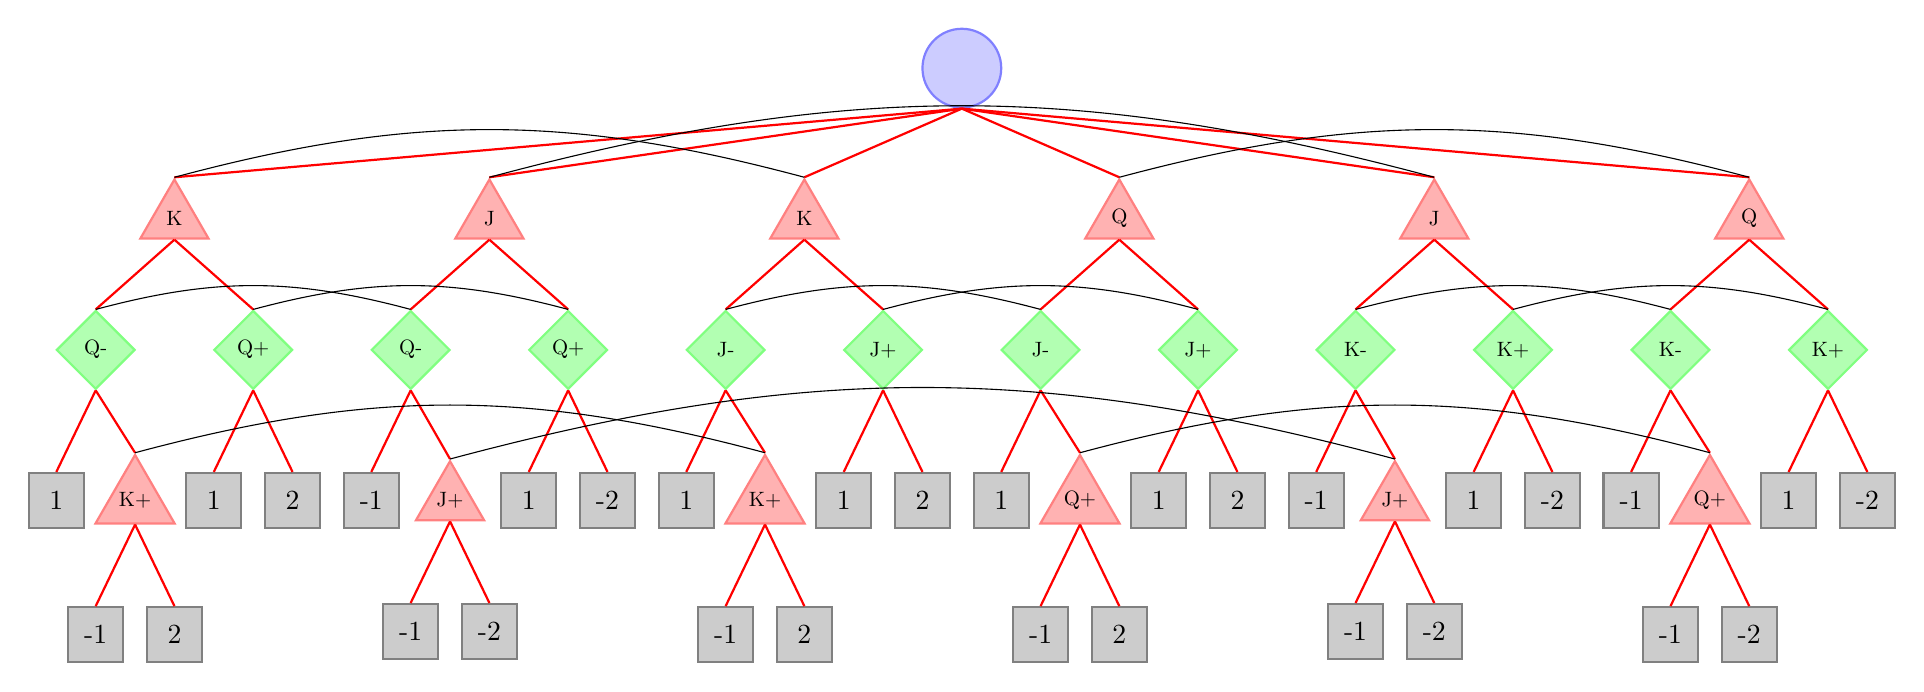
\begin{tikzpicture}
  [chance/.style={circle,draw=blue!50,fill=blue!20,thick,minimum size = 10mm},
   terminal/.style={rectangle,draw=black!50,fill=black!20,thick, minimum size = 7mm},
   maxer/.style={shape=regular polygon, regular polygon sides=3,draw=red!50,fill=red!30,thick,minimum size = 10mm,inner sep = 0pt},
   miner/.style={shape=diamond,draw=green!50,fill=green!30,thick,minimum size = 10mm, inner sep = 0pt},
   edge from parent/.style={red,thick,draw}, 
   parent anchor=south,child anchor=north,
   level 1/.style={sibling distance=4cm,level distance=1.4cm,
       		growth parent anchor=south},
   level 2/.style={sibling distance=2cm},
   level 3/.style={sibling distance=1cm},
   level 4/.style={sibling distance=1.0cm}]
		\node  [chance] {}
		    child {node (M1) [maxer] {\scalebox{.75}{K}}
			child {node (M11) [miner] {\scalebox{.75}{Q-}}
				child {node (M111) [terminal] {1}}
				child {node (M112) [maxer] {\scalebox{.75}{K+}}
					child {node (M1121) [terminal] {-1}}
					child {node (M1122) [terminal] {2}}}
			}
			child {node (M12) [miner] {\scalebox{.75}{Q+}}
				child {node (M121) [terminal] {1}}
				child {node (M122) [terminal] {2}}
			}
		    }
		    child {node (M2) [maxer] {\scalebox{.75}{J}}
			child {node (M21) [miner] {\scalebox{.75}{Q-}}
				child {node (M211) [terminal] {-1}}
				child {node (M212) [maxer] {\scalebox{.75}{J+}}
					child {node (M2121) [terminal] {-1}}
					child {node (M2122) [terminal] {-2}}}
			}
			child {node (M22) [miner] {\scalebox{.75}{Q+}}
				child {node (M221) [terminal] {1}}
				child {node (M222) [terminal] {-2}}
			}
		    }
		    child {node (M3) [maxer] {\scalebox{.75}{K}}
			child {node (M31) [miner] {\scalebox{.75}{J-}}
				child {node (M311) [terminal] {1}}
				child {node (M312) [maxer] {\scalebox{.75}{K+}}
					child {node (M3121) [terminal] {-1}}
					child {node (M3122) [terminal] {2}}}
			}
			child {node (M32) [miner] {\scalebox{.75}{J+}}
				child {node (M321) [terminal] {1}}
				child {node (M322) [terminal] {2}}
			}
		    }
		    child {node (M4) [maxer] {\scalebox{.75}{Q}}
			child {node (M41) [miner] {\scalebox{.75}{J-}}
				child {node (M411) [terminal] {1}}
				child {node (M412) [maxer] {\scalebox{.75}{Q+}}
					child {node (M4121) [terminal] {-1}}
					child {node (M4122) [terminal] {2}}}
			}
			child {node (M42) [miner] {\scalebox{.75}{J+}}
				child {node (M421) [terminal] {1}}
				child {node (M422) [terminal] {2}}
			}
		    }
		    child {node (M5) [maxer] {\scalebox{.75}{J}}
			child {node (M51) [miner] {\scalebox{.75}{K-}}
				child {node (M511) [terminal] {-1}}
				child {node (M512) [maxer] {\scalebox{.75}{J+}}
					child {node (M5121) [terminal] {-1}}
					child {node (M5122) [terminal] {-2}}}
			}
			child {node (M52) [miner] {\scalebox{.75}{K+}}
				child {node (M521) [terminal] {1}}
				child {node (M522) [terminal] {-2}}
			}
		    }
		    child {node (M6) [maxer] {\scalebox{.75}{Q}}
			child {node (M61) [miner] {\scalebox{.75}{K-}}
				child {node (M611) [terminal] {-1}}
				child {node (M612) [maxer] {\scalebox{.75}{Q+}}
					child {node (M6121) [terminal] {-1}}
					child {node (M6122) [terminal] {-2}}}
			}
			child {node (M62) [miner] {\scalebox{.75}{K+}}
				child {node (M621) [terminal] {1}}
				child {node (M622) [terminal] {-2}}
			}
		    };
		\draw  (M1.north) to [dashed,black,out=15,in=165] (M3.north);
		\draw  (M2.north) to [dashed,black,out=15,in=165] (M5.north);
		\draw  (M4.north) to [dashed,black,out=15,in=165] (M6.north);
		\draw  (M112.north) to [dashed,black,out=15,in=165] (M312.north);
		\draw  (M212.north) to [dashed,black,out=15,in=165] (M512.north);
		\draw  (M412.north) to [dashed,black,out=15,in=165] (M612.north);
		\draw  (M11.north) to [dashed,black,out=15,in=165] (M21.north);
		\draw  (M12.north) to [dashed,black,out=15,in=165] (M22.north);
		\draw  (M31.north) to [dashed,black,out=15,in=165] (M41.north);
		\draw  (M32.north) to [dashed,black,out=15,in=165] (M42.north);
		\draw  (M51.north) to [dashed,black,out=15,in=165] (M61.north);
		\draw  (M52.north) to [dashed,black,out=15,in=165] (M62.north);
\end{tikzpicture}
} %scalebox
\caption{}
\label{fulltree}
\end{figure}

Table~\ref{sampletimes}
\begin{table}
\begin{tabular}{ccc}
1 & 18 & 0.000\\
2 & 18 & 0.000\\
3 & 18 & 0.000\\
4 & 279 & 0.008\\
5 & 242 & 0.028\\
6 & 216 & 0.052\\
7 & 176 & 0.064\\
8 & 3406 & 0.092\\
9 & 2191 & 0.288\\
10 & 1423 & 0.508\\
11 & 1363 & 0.596\\
12 & 1416 & 0.744\\
13 & 1416 & 0.836\\
14 & 3440 & 0.97\\
15 & 3428 & 1.25\\
16 & 50521 & 1.82\\
17 & 43192 & 5.91\\
18 & 26128 & 7.94\\
19 & 19061 & 9.92\\
\end{tabular}
\caption{Solution counts and running times for a sample kriegspiel game}
\label{white times}
\end{table}

Table~\ref{sampletimes}
\begin{table}
\begin{tabular}{ccc}
1 & 20 & .000\\
2 & 19 & .000\\
3 & 404 & .008\\
4 & 401 & .024\\
5 & 1472 & .044\\
6 & 155 & .096\\
7 & 293 & .116\\
8 & 158 & .128\\
9 & 118 & .148\\
10 & 25 & .152\\
11 & 798 & .164\\
12 & 518 & .192\\
13 & 13564 & .304\\
14 & 12394 & .776\\
15 & 343652 & 3.75\\
16 & 320704 & 17.3\\
17 & 490162 & 99.9\\
18 & 3792 & 119\\
19 & 14836 & 121 \\
\end{tabular}
\caption{Solution counts and running times for a sample kriegspiel game}
\label{blacktimes}
\end{table}




%\nocite{*}
\nocite{richards09information}
\nocite{russell05efficient}
\nocite{kuhn03lectures}
\nocite{kuhn97classics}
\nocite{parker05sampling}
\nocite{nance06reasoning}
\nocite{li94chess}

\bibliographystyle{acm}
\bibliography{paper}
%\begin{thebibliography}{99}
%\end{thebibliography}

\end{document}
